\section{Preliminary}
\label{sec:preliminary}

% In this section, we introduce how to inject noise signal into recording devices without disturbing the people around, then we describe the linguistic structure of speech signals and how they are understood by speech recognition system and human auditory system.

In this section, we introduce the nonlinearity effect in the microphone, then we describe the linguistic structure of speeches and how humans and machines understand them.

\subsection{Nonlinearity in Microphone}
% \subsection{Jamming with the Nonlinearity in Microphone}
A microphone is a type of transducer that converts acoustic signals into electrical signals. Previous studies have shown that the preamplifier in most types of microphones, including Electret Condenser Microphones (ECMs) and Micro Electro Mechanical Systems (MEMS) Microphones, involves nonlinear operations that cause inter-modulation distortion in its output \cite{7569908}. As a result, the microphone's output contains both frequency components of the input and all possible linear combinations of them \cite{zi-qiang_lang_evaluation_2000}. To illustrate, suppose the inputs are two single tones with frequencies of $f_1$ and $f_2$, the nonlinearity makes the output contain not only components with frequencies of $f_1, f_2$, but also $f_1+f_2$, $f_1-f_2$, $2f_1$, $2f_2$, ... etc., as shown in the left of Figure~\ref{fig:nonlinearity_in_microphone}.

\begin{figure}[t]
    \centering
    \begin{subfigure}[b]{0.49\columnwidth}
        \centering
        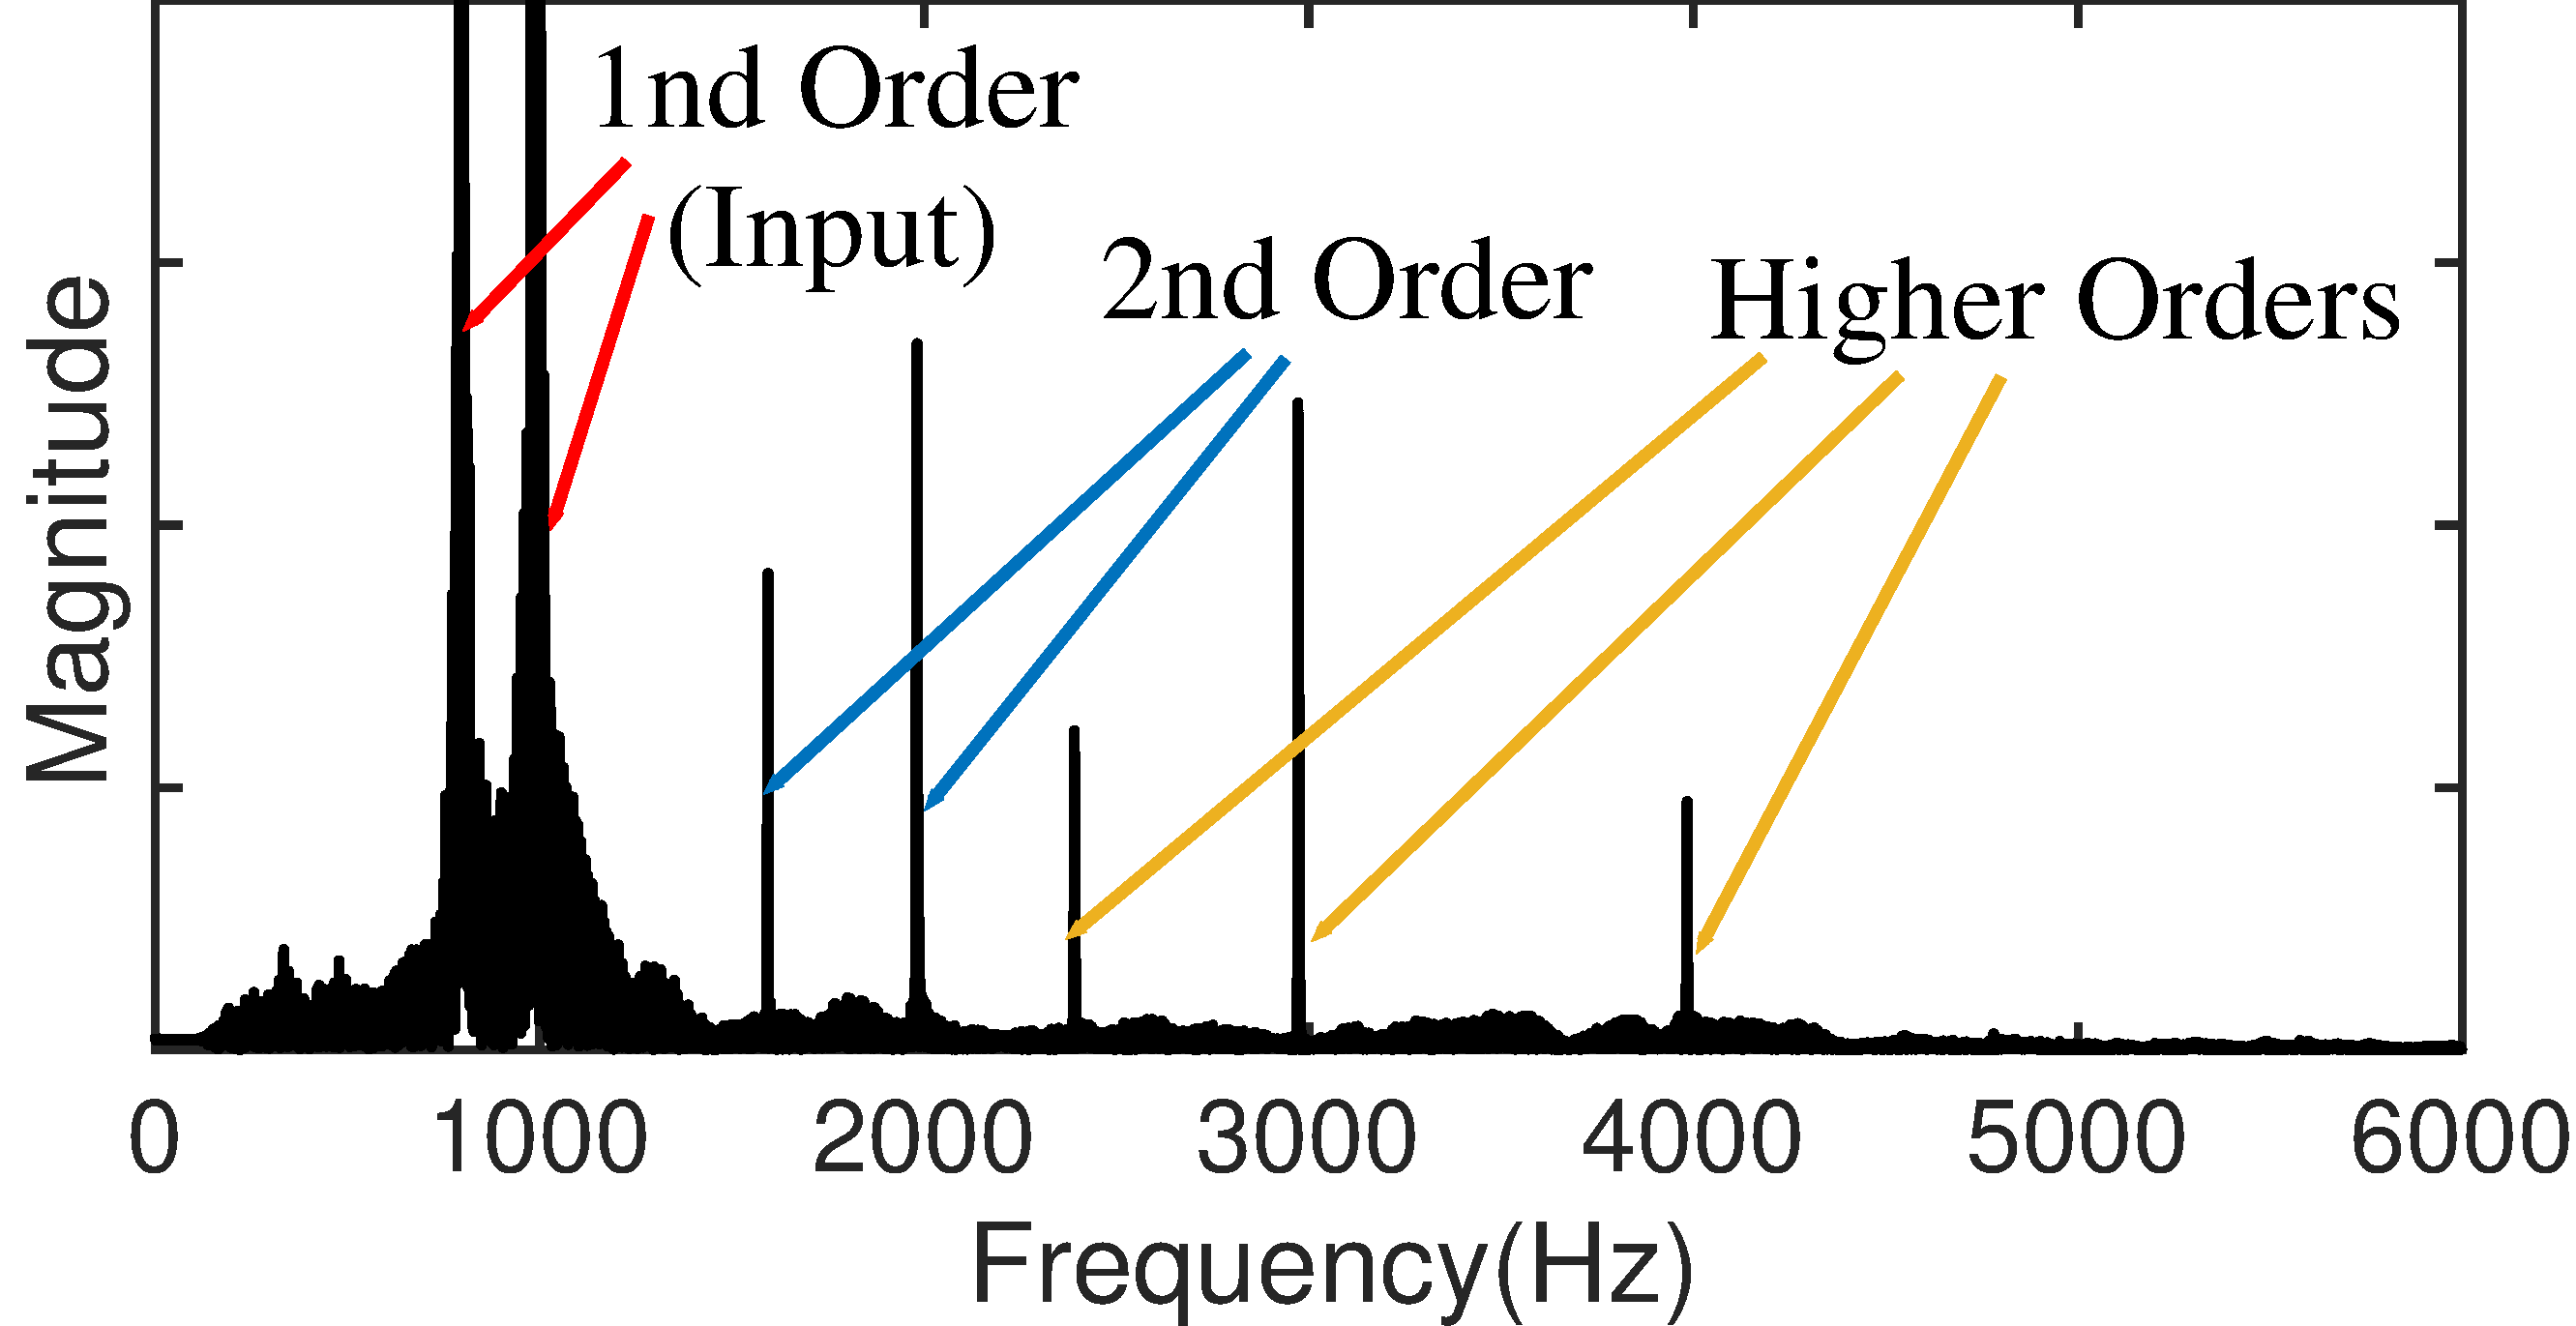
\includegraphics[width=\linewidth]{images/interModulation.pdf}
    \end{subfigure}
    \begin{subfigure}[b]{0.49\columnwidth}
        \centering
        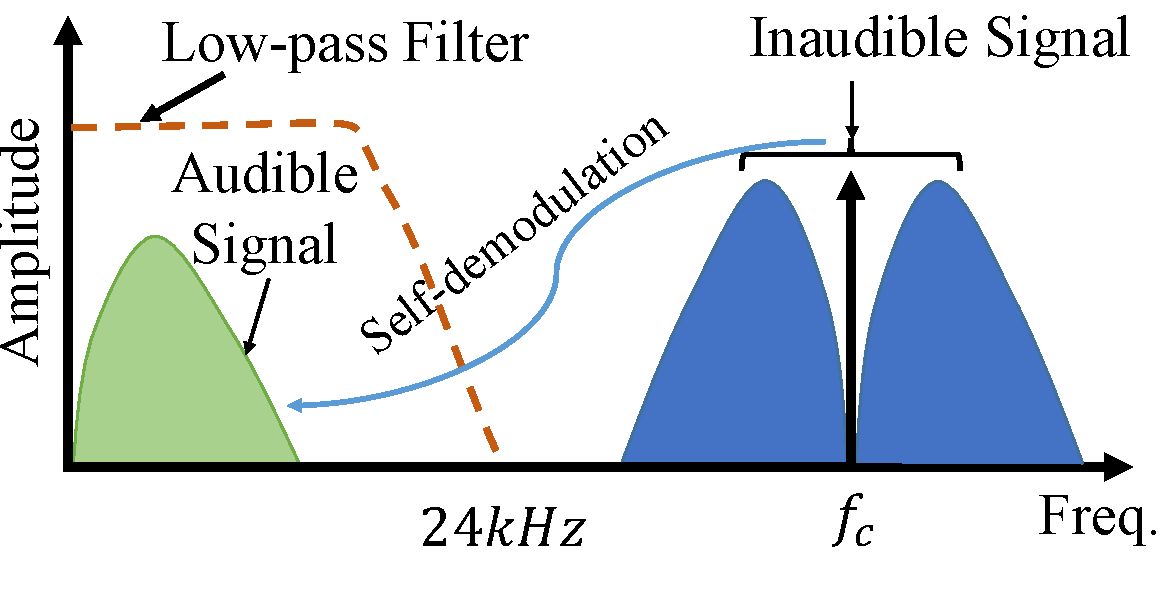
\includegraphics[width=\linewidth]{images/voiceTransmission.pdf}
    \end{subfigure}
    \caption{Nonlinearity in microphone. The left figure shows the audio spectrum recorded by a Huawei P10 smartphone with an input of two single tones (800Hz and 1000Hz).}

    \label{fig:nonlinearity_in_microphone}
    \vspace{-5mm}
\end{figure}

To inject an audible noise signal $n(t)$ into a microphone stealthily, we first modulate $n(t)$ on a high-frequency carrier $c(t)$ = $cos(2\pi f_c t)$ via amplitude modulation and then transmit the modulated signal along with the carrier simultaneously. When these signals arrive at a microphone, the non-linearity produces distortion that are harmonics and cross-products of the carrier and the modulated noise~\cite{10.1145/3133956.3134052}, generating a low-frequency shadow signal and other high frequency components. The shadow signal is the same as $n(t)$ and other components will be filtered out by the low-pass filter in the microphone, as shown Figure~\ref{fig:nonlinearity_in_microphone} (right part).

\subsection{Informational Masking}
\label{subsec:informational_masking}
Informational masking, which is first defined in~\cite{Pollack1975-qm}, describes the degradation of the auditory detection threshold in the human brain when the target sound is embedded in other interferers with similar characteristics. Informational masking is usually associated with its complementary term: energetic masking, which occurs when interferers are present at the same time and the same frequency bands~\cite{leek_informational_1991}. Unlike energetic masking which mainly depends on the relative energy between the target and the interferer in each frequency band, the degree of information masking mainly depends on the similarity between the target and the interferer. Generally speaking, these two types of masking are not independent and they always affect the auditory detection threshold simultaneously.


\subsection{Human Auditory System and ASR}
\label{subsec:human_auditory_system_and_asr}
One of the main tasks of the human auditory and ASR systems is extracting semantic information from speech signals. In order to improve speech intelligibility, both systems need to first eliminate the noise in the signals, then extract phoneme series, the primary component of a speech signal, and decode the phoneme sequence into meaningful content. 

The attention mechanism in the human auditory system, as known as "Cocktail Party Effect", has a strong noise reduction ability~\cite{festen_effects_1990, leek_informational_1991,brungart_informational_2001, mattys_effects_2010}. It allows a listener to distinguish signals from other sources and then eliminates the influence of uninterested noises, thus achieving denoising. To be more vivid, imagine you are whispering to a friend in a crowded cocktail bar where many people are talking loudly, although other people's voices may be louder than your friend's, you can still focus on his/her voice and understand what he/she is talking about. This mechanism also helps human beings to reduce the impact of masking effect caused by interferences. The effectiveness of the attention mechanism mainly depends on the degree of difference between the target signal and the noise in three aspects: fundamental frequency, temporal properties, and spatial distribution. A larger difference means better discrimination with the help of the attention mechanism.

A typical ASR system works similarly to the human auditory system to "comprehend" speech signals. Most of these ASR systems will first extract voice features, such as mel-frequency cepstral coefficients (MFCC), from the audio segments and then recognize the phoneme series from these features using an acoustic model. Then with the help of the pronunciation model and language model, the phoneme series will be decoded into normal text. To improve recognition accuracy, speech enhancement methods are always applied before recognition. 
The widely used speech enhancement methods can be roughly divided into two types: noise reduction and noise separation. The former, such as spectral subtraction, targets on reducing the noise from the signals. This type of method relies on the invariance of statistical characteristics of noise and the differences in temporal properties between the noise and the target speech signal. The noise separation, such as blind signal separation, targets on separating source signals from mixed signals. Such methods rely on the assumption that each source signal is independent. 

In this work, we aim to prevent both humans and machines from extracting semantic information embedded in speech signals by injecting noise signals into the recordings. To achieve this target, the injected noise should interfere with human and ASRs' understanding of semantics. Equally critical, the injected noise should be difficult to remove by both auditory attention mechanism and speech enhancement algorithms. Therefore, we design our noise that is highly correlated with speech signals to affect the phoneme structure of the target speech signal, which not only disturbs human's and ASR's understanding of the semantics, but also improves the robustness of noise against speech enhancement methods.

